\section{Redux}
\subsection{Flux}

In klassischen Architekturen wie MVC und MVVM ist der State in den entsprechenden Models verteilt. Der State ist innerhalb der Applikation stark fragmentiert. Als Antwort zur Fragmentierung entstand ein neuer Trend in SPA hin zu den One-Way Data Flow Patterns. Daten fliessen in Form von Nachrichten in einer Richtung durch die Applikation.  Der State wird zentral im Store verwaltet. Ein Vorreiter der One-Way Data Flow Pattern ist Flux von Facebook. Innerhalb von Flux kann es beliebig viele Stores, Actions und Views geben, jedoch nur einen Dispatcher.

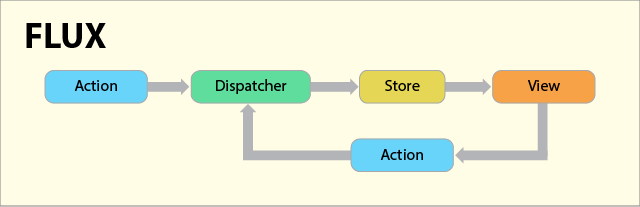
\includegraphics[width=\columnwidth]{images/flux}

\subsection{Redux}
Redux setzt das One-Way Data Flow Patterns um. Eine Redux-Applikation kennt genau einen einzigen Store. Im Store wird der komplette State der Anwendung zentral gespeichert wird. Aktionen stellen (wie bei Flux) die einzige Möglichkeit dar, den State im Store zu verändern. Um zu definieren, wie genau diese Änderungen funktionieren, gibt es das Konzept der Reducer. Reducers sind als sogenannte "Pure Functions" realisiert, JavaScript-Funktionen ohne Seiteneffekte => funktionale Programmierung.

\subsubsection{Die 3 Kernprinzipien von Redux}
\textbf{Single source of truth}
Der Zustand der Anwendung wird zentral über einen einzigen Store gemanagt.

\textbf{State is read-only}
Die Anwendung reagiert auf Benutzerinteraktionen, indem sie mit einem ActionCreator eine Action erzeugt, die anzeigt, was gerade passiert ist. Mit einem Reducer wird dann abhängig von der Action aus dem alten Zustand ein neuer Zustand erzeugt.

\textbf{Changes are made with pure functions}
Reducer sind seiteneffektfreie Funktionen. Sie erhalten zwei Eingabeparameter (den derzeitigen Anwendungszustand sowie die Action, die gerade ausgelöst wurde) und erzeugen daraus eine Ausgabe (den neuen Anwendungszustand).

\subsubsection{Schlüsselkonzepte}

\begin{itemize}
	\item Alle Applikationsdaten werden über eine einzige Datenstruktur, genannt State, im Store verwaltet.
	\item Die Applikation liest den State immer aus dem Store.
	\item Der State wird nie ausserhalb des Stores verändert.
	\item Ein View kann eine Action auslösen, die beschreibt was passieren soll.
	\item Der neue State wird in sogenannten Reducer aus dem alte State und der Action neu bestimmt.
\end{itemize}

\subsubsection{Datenfluss}

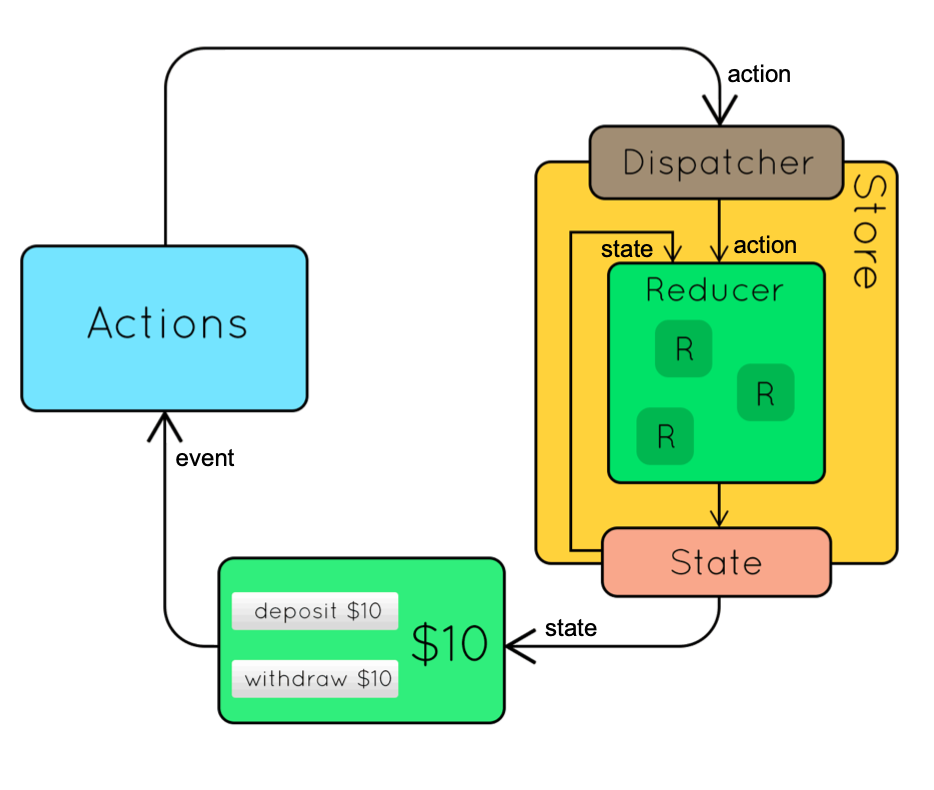
\includegraphics[width=\columnwidth]{images/datenfluss}

\subsubsection{Reducers}

In einer grossen Applikation müssen sehr viele unterschiedliche Aspekte als State im Store verwaltet werden. Deshalb ist es notwendig, dass das Konzept "Reducer" skaliert, so dass ein Reducer überblickbar bleibt.
Eine Aufteilung in mehrere Reducers wird von Redux unterstützt, wobei jeder Reducer für die Verwaltung eines konkreten State- Aspekt verantwortlich ist.
In Redux müssen diese Reducers schlussendlich zusammengefasst werden mit: redux.combineReducers({reducer1, reducer2, ...})

\subsection{Code}
\begin{minted}{javascript}
const redux = require('redux')
const logFactory = require('redux-logger')
const thunk = require('redux-thunk').default

const logger = logFactory.createLogger({
    colors: false
});

function counterReducer(state = 0, action) {
    switch (action.type) {
        case 'INCREMENT':
            return state.counter + 1
        case 'DECREMENT':
            return state.counter - 1
        default:
            return state
    }
}


function waitingReducer(state = false, action) {
    switch (action.type) {
        case 'WAITING':
            return true
        case 'RUNNING':
            return false
        default:
            return state
    }
}

function incrementAsync() {
    return (dispatch) => {
        dispatch({type: 'WAITING'})
        setTimeout(() => {
            dispatch({type: 'RUNNING'})
            dispatch({type: 'INCREMENT'})
        }, 2000);
    }
}

const reducers = redux.combineReducers({ counter: counterReducer,
    waiting: waitingReducer
})

let store = redux.createStore(reducers, redux.applyMiddleware(thunk, logger));

store.subscribe(() => console.log("The actual state counter is " + store.getState()))

store.dispatch({type: 'INCREMENT'})
store.dispatch(incrementAsync())
store.dispatch({type: 'INCREMENT'})
store.dispatch({type: 'DECREMENT'})
\end{minted}

\subsection{Beispiel Filme}
\subsubsection{index.js}
\begin{minted}{javascript}
const ACTIONS = {
    'UPDATE_FILTER_TERM': (state, action) => ({ ...state, filterTerm: action.filterTerm })
}

const reducer = (state, action) => _.get(ACTIONS, action.type, _.identity)(state, action)

const initialState = {
    movies: [
        {rank: 1, title: 'The Shawshank Redemption', director: 'Frank Darabont', year: 1994},
        {rank: 2, title: 'The Godfather', director: 'Francis Ford Coppola', year: 1972},
        {rank: 3, title: 'The Dark Knight', director: 'Christopher Nolan', year: 2008},
        {rank: 4, title: 'The Godfather: Part II', director: 'Francis Ford Coppola', year: 1974},
        {rank: 5, title: 'The Lord of the Rings: The Return of the King', director: 'Peter Jackson', year: 2003},
        {rank: 6, title: 'Pulp Fiction', director: 'Quentin Tarantino', year: 1994},
        {rank: 7, title: 'Schindlers List', director: 'Steven Spielberg', year: 1993},
        {rank: 8, title: '12 Angry Men', director: 'Sidney Lumet', year: 1957},
        {rank: 9, title: 'Fight Club', director: 'David Fincher', year: 1999}
    ],
    filterTerm: ''
}

const store = createStore(reducer, initialState)

ReactDOM.render(
    <Provider store={store}>
        <App/>
    </Provider>,
    document.getElementById('app')
)
\end{minted}

\subsubsection{App.js}

\begin{minted}{javascript}
const filter = (movies, term) => {
    let filterTerm = '^(?=.*' + _.trim(term).split(/\s+/).join(')(?=.*') + ').*$'
    let pattern = RegExp(filterTerm, 'i')

    return _.filter(movies, movie =>
        pattern.test(_.join([movie.year, movie.director, movie.title], ' ')))
}

const App = () => {
    const movies = useSelector(state => state.movies, _.isEqual)
    const filterTerm = useSelector(state => state.filterTerm, _.isEqual)
    const dispatch = useDispatch()

    const updateFilterTerm = term =>
        dispatch({ type: 'UPDATE_FILTER_TERM', filterTerm: term })

    return <main>
        <Filter term={ filterTerm } updateFilterTerm={ updateFilterTerm } />
        { _.map(filter(movies, filterTerm), movie => <Movie key={ movie.rank } data={ movie } />) }
    </main>
}

export default App
\end{minted}

\subsubsection{Filter.js}

\begin{minted}{java}
const Filter = ({ filterTerm }) => {
    const dispatch = useDispatch()

    const onChange = event =>
        dispatch({ type: 'UPDATE_FILTER_TERM', filterTerm: event.target.value })

    return <form>
        <input type='text' placeholder='Liste Filtern mit...' value={ filterTerm } onChange={ onChange } />
    </form>
}

export default Filter
\end{minted}

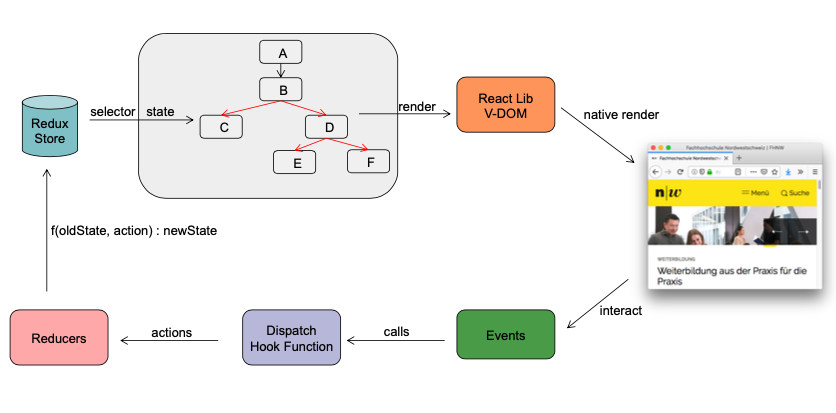
\includegraphics[width=\columnwidth]{images/reduxflow}

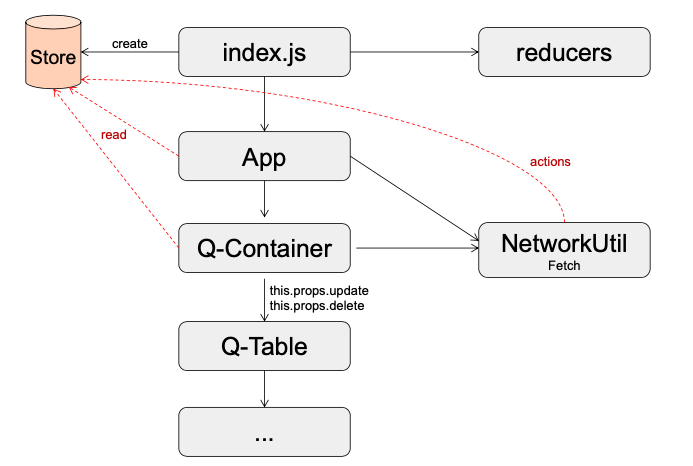
\includegraphics[width=\columnwidth]{images/flashcardredux}

